%!TEX root = ../seminararbeit.tex
\newpage
\section{SAP Analytics Cloud}\label{sec:sac}
Um die Kriterien zur Ideenbewertung bei \ac{sac} zu analysieren, ist es zunächst 
wichtig, ein Verständnis über den grundlegenden Aufbau, die Arbeitsweise sowie Hintergründe bezüglich 
existierender Kunden zu erhalten. 

\subsection{Produktbeschreibung}
\ac{sac} ist eine Anwendung, die es ermöglicht Analysen, Planungen und Prognosen in einer einzigen Anwendung durchzuführen. 
\begin{figure}[ht]
	\centering 
	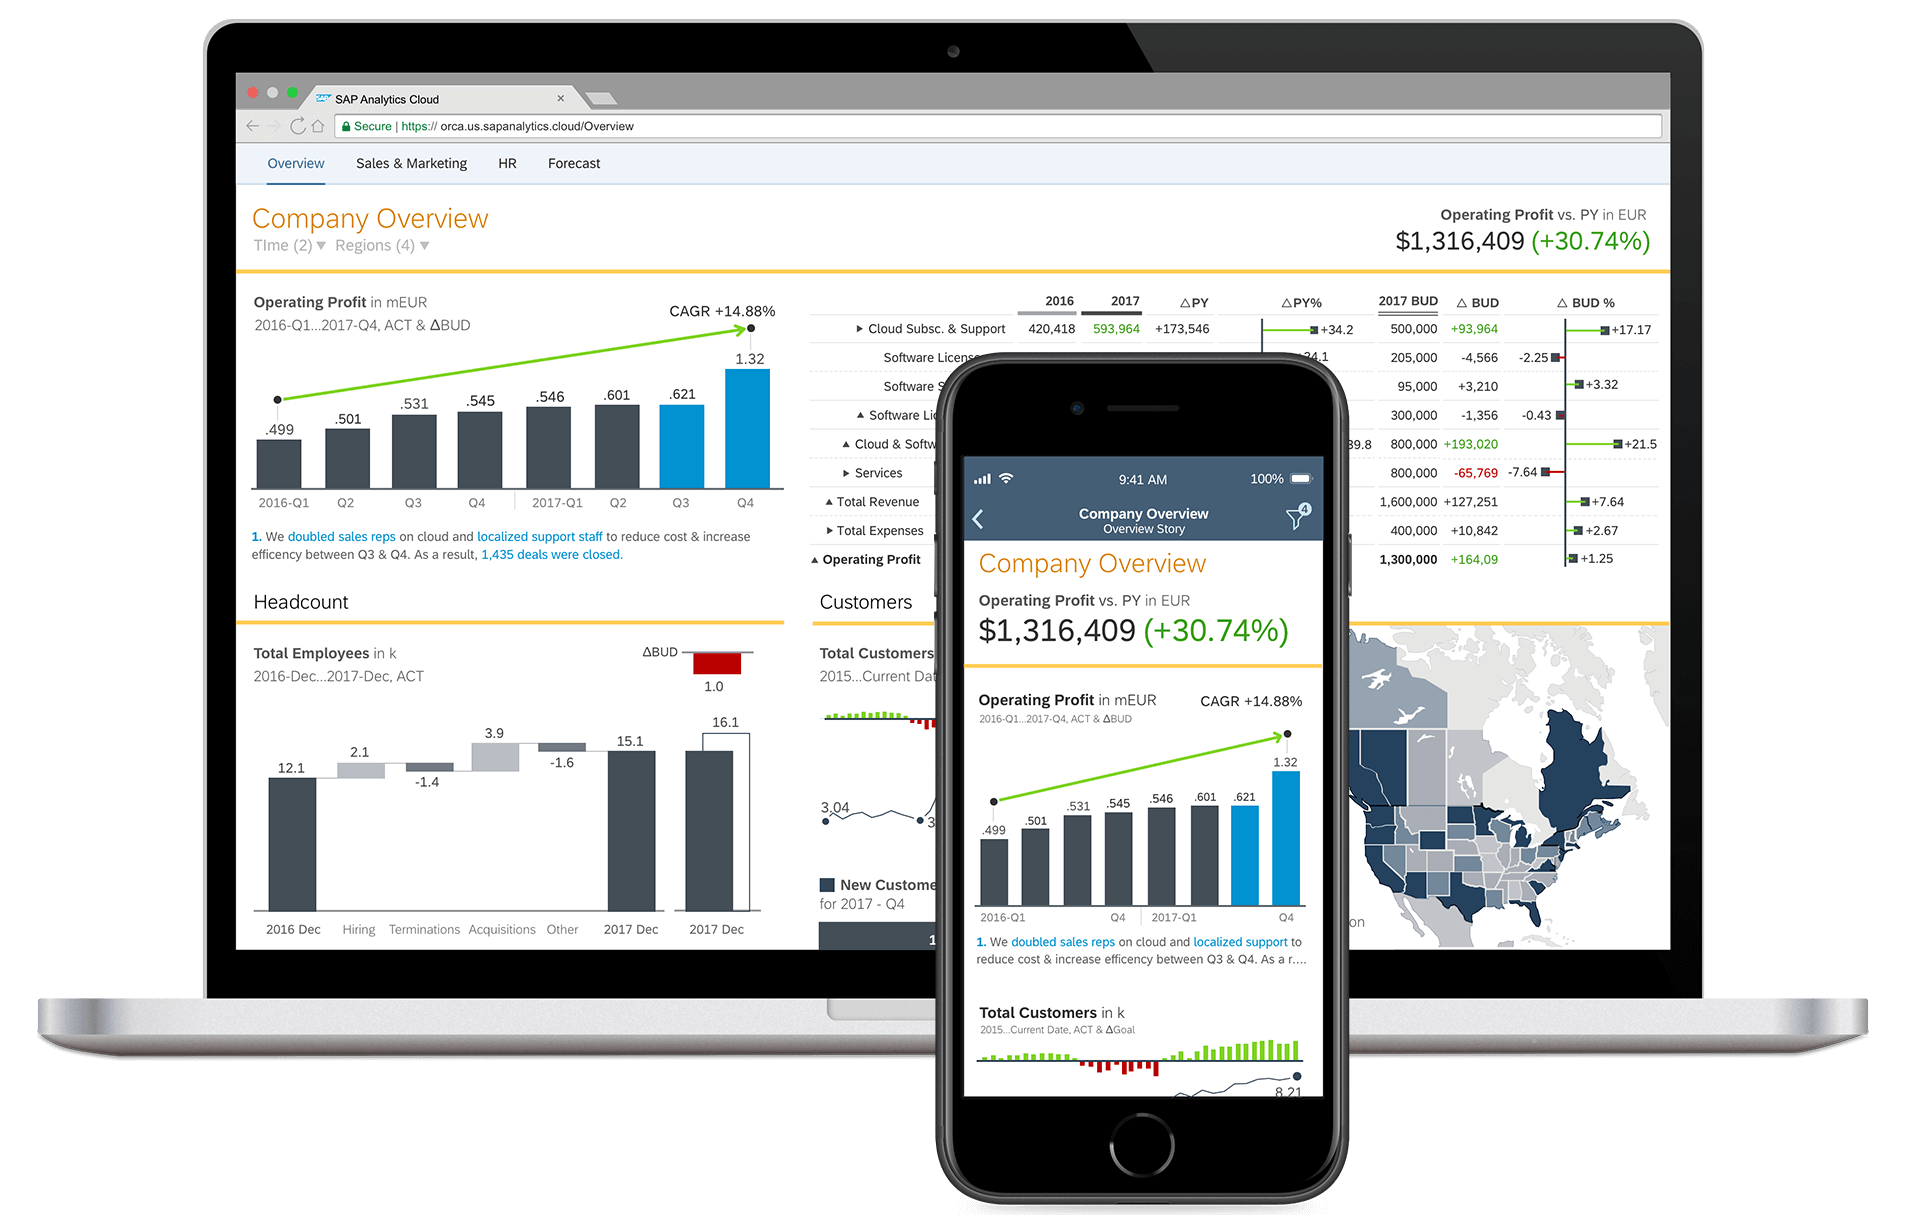
\includegraphics[width=7cm]{homehero.png}
	\caption{SAP Analytics Cloud}
	\label{img:homeHeroSAC}
\end{figure}
Die gesamte Applikation enthält sehr viele Funktionalitäten, die den Rahmen dieser Seminararbeit sprengen würden. Dennoch ist
es sinnvoll über die Grundfunktionalitäten des Produkts bescheid zu wissen. 
Grundsätzlich arbeitet \ac{sac} in drei Schritten. 

\begin{enumerate}
    \item Daten zur Verfügung stellen
    \item Modellierung der Informationen
    \item Auswertung und Verwendung der gewonnen Informationen 
\end{enumerate}
Der letzte Schritt ermöglicht das Analysieren der Informationen und das Planen. 

\subsection{Aufbau der Abteilung}
Die Abteilung die das Product \ac{sac} entwickelt, besteht aus weltweit verteilten Teams, 
die Verantwortung für verschiedene Bereiche des Produkts besitzen und diese entwickeln. 
Die beiden Hauptstandorte sind Vancouver in Kanada und Walldorf in Deutschland. Weitere Teams sind beispielsweise in 
Shanghai oder Bangalore. Besonders bei globalen Entwicklungen ist es wichtig, Ideen bereits vorbewertet an andere Teams 
heranzutragen, denn der Kommunikationsaufwand zwischen mehreren Kontinenten ist kein zu unterschätzender Kostenfaktor. 
Die Struktur der Abteilung ist streng hierarchisch. Das bedeutet, dass viele Ideen bereits von Managern diskutiert und 
bewertet wurden bevor sie bis zum Entwickler durchgereicht werden. Dennoch hat auch der Entwickler die Herausforderung, 
mehrere Ideen zu bewerten und abzuwägen welche dieser Ideen umgesetzt werden soll. Dabei handelt es sich meist, um detailierte Umsetzungsmöglichkeiten
einer Anforderung. 
Neben den Managern und Entwicklern besitzt die Abteilung außerdem Designer, die Oberflächen-Mockups entwickeln und auf
die \ac{ux} achten. Zuletzt, aber besonders wichtig sind die Qualitätsverantwortlichen der Abteilung. Diese 
arbeiten mit den Entwicklern zusammen um durch Testkonzepte die Qualität des Produkts zu gewährleisten.

\subsection{Existierende Kunden}
Das Produkt war lange Zeit ausschließlich in der Entwicklung, wird seit einigen Jahren jedoch produktiv von Kunden verwendet. Besonders 
interessant im Bezug auf die Ideenbewertung sind einige wenige aber wichtige Kunden, die sich durch Feedback in die 
Weiterentwicklung des Produkts einbringen. Diese Kunden melden zurück, welche Funktionen für sie sinnvoll oder 
zwingend notwendig sind. Sie haben so direkten Einfluss auf die Ideenbewertung. 

\subsection{Arbeitsweise in der Abteilung}
Die Abteilung arbeitet in einem individualisertem Scrum-Modus. Scrum ist eine agile Prozessmethode und basiert 
auf dem Grundsatz, dass viele kleine Pakete einfacher zu entwickeln sind, als ein großes Paket. 
\begin{quote} Scrum basiert,[...], auf der Erkenntnis, daß es wesentlich einfacher ist, einen kleinen Bissen zu verdauen als einen großen.\cite{scrum:2018} \end{quote} 
Der Kern von Scrum sind die vergleichsweise kurzen \textit{Sprints}, nach denen ein Entwicklungspaket implementiert wurde. 
In \ac{sac} haben diese Sprints eine Länge von zwei Wochen. Dies bedeutet allerdings nicht, dass ein Paket 
innerhalb dieser Zeit fertiggestellt werden muss. 
Bei Funktionen, die von mehreren Teams entwickelt werden, sind meist mehrere Sprints für die Entwicklung eingeplant um den Aufwand für die Kommunikation zu berücksichtigen. 
Nach der Fertigstellung eines Entwicklungspakets wird ein weiterer Sprint zum Stabilisieren und Testen angehängt, bevor die Funktionalität an einen Kunden
ausgeliefert wird. \autoref{img:sac-sprint} zeigt einen Ausschnitt der Sprint-Planung.
Damit eine Funktionalität als \textit{bereit für die Auslieferung zum Kunden} gilt, müssen Manager, Designer und Qualitätsverantwortlichen das 
Einverständnis geben. Dieses Konzept wird bei Scrum als \ac{dod} bezeichnet. 
\begin{figure}[ht]
	\centering
	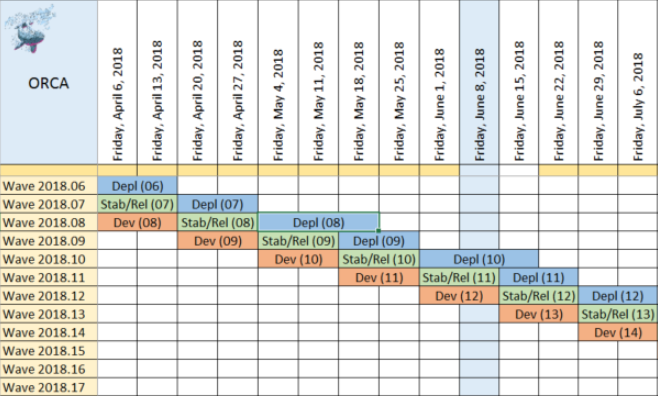
\includegraphics[width=10cm]{sprints.png}
	\caption{Sprintüberblick}
	\label{img:sac-sprint}
\end{figure}



\subsection{Team: Modeling}
Das Modeling-Team ist für einen Bereich der Anwendung verantwortlich, der viele Schnittpunkte zu anderen Teams besitzt.
Einige dieser Schnittstellen sind in \autoref{img:sac-modeling} dargestellt. Wrangling ist hauptsächlich für das 
Einbinden von Datenquellen verantwortlich. Sie sorgen dafür, dass ein Kunde aus verschiedenen Quellen Modelle erstellen kann oder Daten in 
ein existierendes Modell laden kann. 
\begin{figure}[ht]
	\centering
	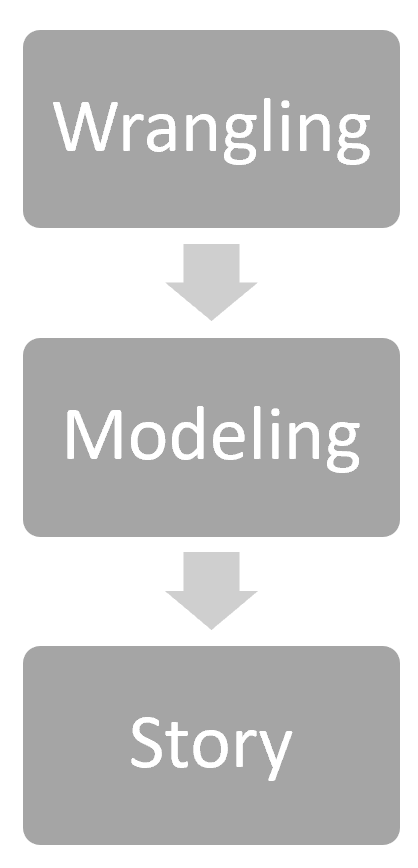
\includegraphics[width=2cm]{modeling.png}
	\caption{Schnittstellen zu Modeling}
	\label{img:sac-modeling}
\end{figure}

Modelle stellen die Struktur der Daten da und konstruieren aus diesen Daten Informationen. Dies ist die Aufgabe des Modeling Teams.
Im Modelingbreich lassen sich, neben vielen weiteren Funktionalitäten, verschiedene Dimensionen, Maßstäbe und Formeln definieren.
Eine dieser Dimensionen, die Account Dimension, wird in \autoref{img:sac-accdim} gezeigt. 
Anhand dieser Strukturierungsinformationen werden die Daten als Informationen in der Story angezeigt.
\begin{figure}[ht]
	\centering
	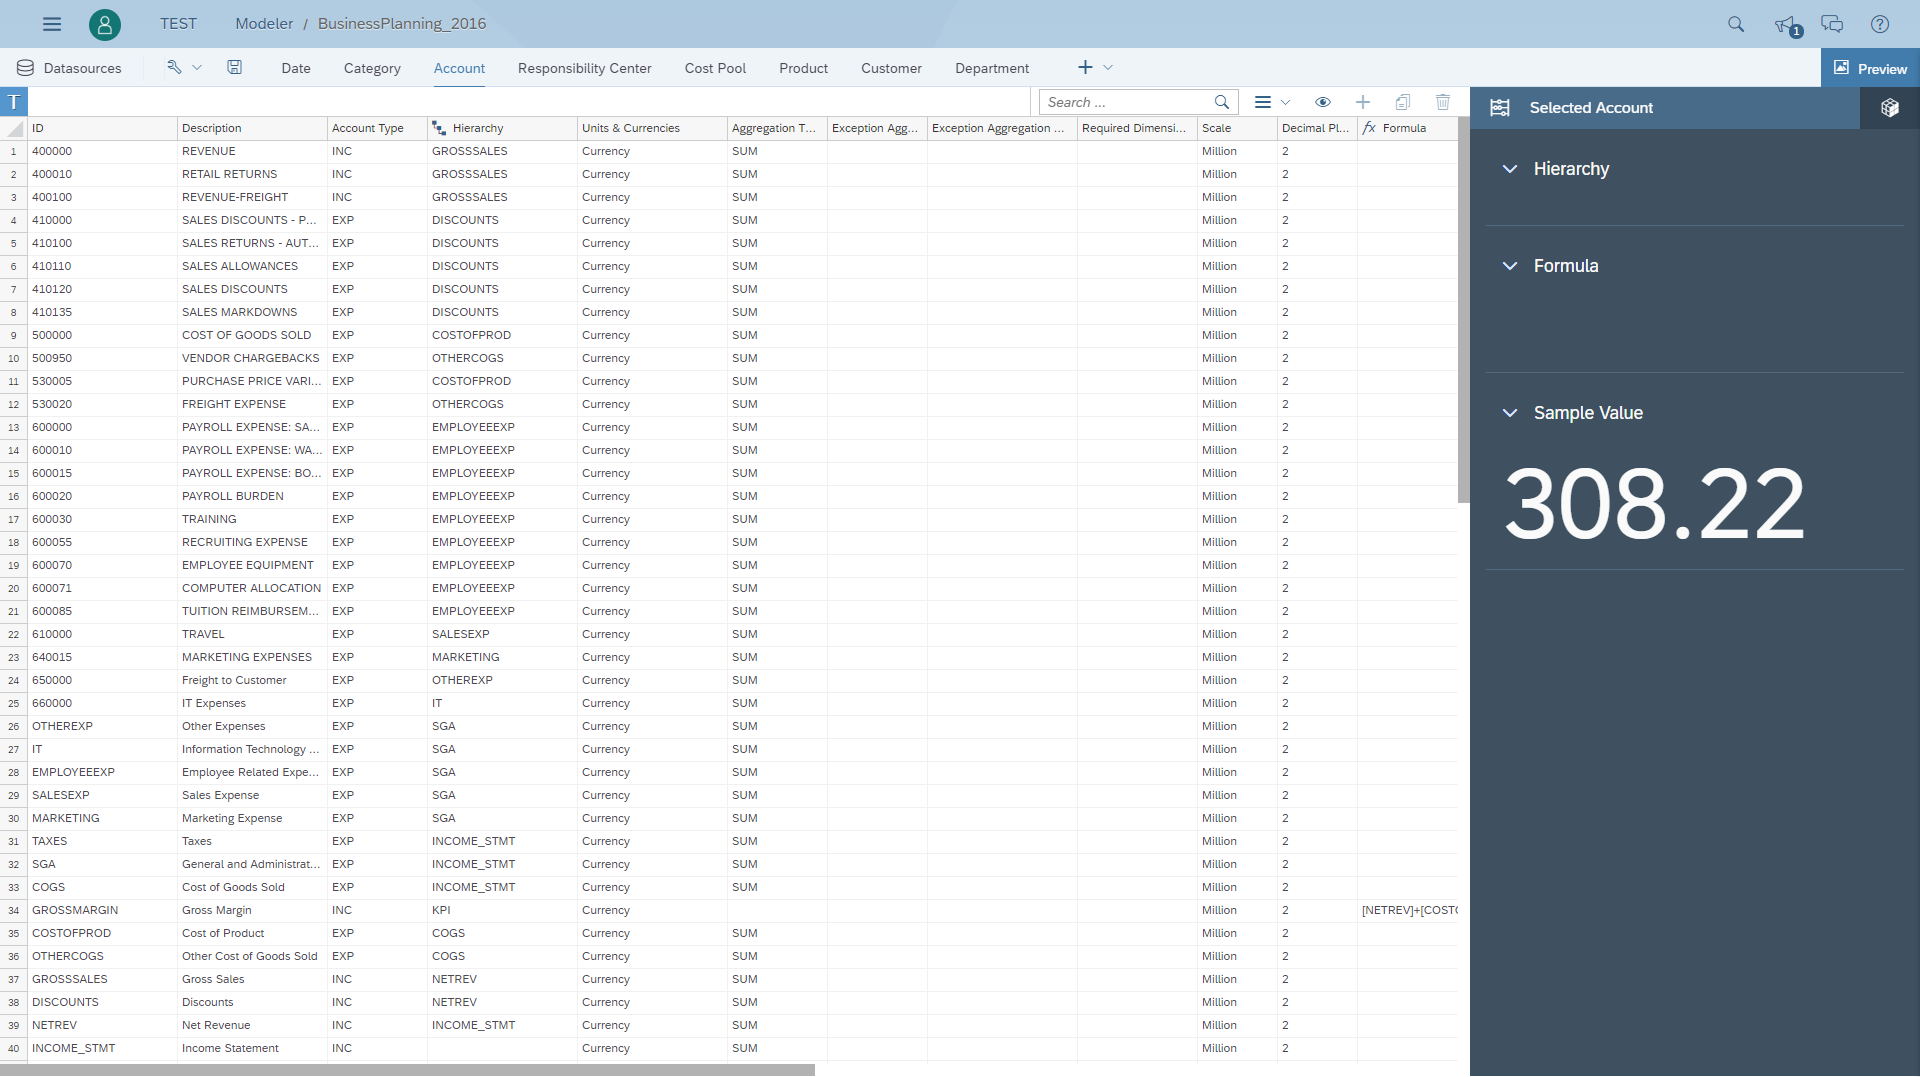
\includegraphics[width=14cm]{accdim.png}
	\caption{Account-Dimension eines Testmodels}
	\label{img:sac-accdim}
\end{figure}

% Das Modeling besteht neben einem Manager aus zwei Architekten, die den Manager mit der Entscheidung über 
% Entwicklungsaufgaben unterstützen und den gesamten Modeling-Bereich technisch überblicken. Außerdem gibt es zwei Designer 
% die Vorschläge für das \ac{ui} erstellen und bei der \ac{ux} unterstützen. Zuletzt gibt es zwei Qualitätsverantwortliche, die den Entwickler 
% beim Testen unterstützen und die Qualität des Produkts überprüfen. 

